\documentclass[]{article}
\usepackage{lmodern}
\usepackage{amssymb,amsmath}
\usepackage{ifxetex,ifluatex}
\usepackage{fixltx2e} % provides \textsubscript
\ifnum 0\ifxetex 1\fi\ifluatex 1\fi=0 % if pdftex
  \usepackage[T1]{fontenc}
  \usepackage[utf8]{inputenc}
\else % if luatex or xelatex
  \ifxetex
    \usepackage{mathspec}
  \else
    \usepackage{fontspec}
  \fi
  \defaultfontfeatures{Ligatures=TeX,Scale=MatchLowercase}
\fi
% use upquote if available, for straight quotes in verbatim environments
\IfFileExists{upquote.sty}{\usepackage{upquote}}{}
% use microtype if available
\IfFileExists{microtype.sty}{%
\usepackage{microtype}
\UseMicrotypeSet[protrusion]{basicmath} % disable protrusion for tt fonts
}{}
\usepackage[margin=1in]{geometry}
\usepackage{hyperref}
\hypersetup{unicode=true,
            pdftitle={DATA605 Discussion 13},
            pdfauthor={Henry Otuadinma},
            pdfborder={0 0 0},
            breaklinks=true}
\urlstyle{same}  % don't use monospace font for urls
\usepackage{color}
\usepackage{fancyvrb}
\newcommand{\VerbBar}{|}
\newcommand{\VERB}{\Verb[commandchars=\\\{\}]}
\DefineVerbatimEnvironment{Highlighting}{Verbatim}{commandchars=\\\{\}}
% Add ',fontsize=\small' for more characters per line
\usepackage{framed}
\definecolor{shadecolor}{RGB}{248,248,248}
\newenvironment{Shaded}{\begin{snugshade}}{\end{snugshade}}
\newcommand{\AlertTok}[1]{\textcolor[rgb]{0.94,0.16,0.16}{#1}}
\newcommand{\AnnotationTok}[1]{\textcolor[rgb]{0.56,0.35,0.01}{\textbf{\textit{#1}}}}
\newcommand{\AttributeTok}[1]{\textcolor[rgb]{0.77,0.63,0.00}{#1}}
\newcommand{\BaseNTok}[1]{\textcolor[rgb]{0.00,0.00,0.81}{#1}}
\newcommand{\BuiltInTok}[1]{#1}
\newcommand{\CharTok}[1]{\textcolor[rgb]{0.31,0.60,0.02}{#1}}
\newcommand{\CommentTok}[1]{\textcolor[rgb]{0.56,0.35,0.01}{\textit{#1}}}
\newcommand{\CommentVarTok}[1]{\textcolor[rgb]{0.56,0.35,0.01}{\textbf{\textit{#1}}}}
\newcommand{\ConstantTok}[1]{\textcolor[rgb]{0.00,0.00,0.00}{#1}}
\newcommand{\ControlFlowTok}[1]{\textcolor[rgb]{0.13,0.29,0.53}{\textbf{#1}}}
\newcommand{\DataTypeTok}[1]{\textcolor[rgb]{0.13,0.29,0.53}{#1}}
\newcommand{\DecValTok}[1]{\textcolor[rgb]{0.00,0.00,0.81}{#1}}
\newcommand{\DocumentationTok}[1]{\textcolor[rgb]{0.56,0.35,0.01}{\textbf{\textit{#1}}}}
\newcommand{\ErrorTok}[1]{\textcolor[rgb]{0.64,0.00,0.00}{\textbf{#1}}}
\newcommand{\ExtensionTok}[1]{#1}
\newcommand{\FloatTok}[1]{\textcolor[rgb]{0.00,0.00,0.81}{#1}}
\newcommand{\FunctionTok}[1]{\textcolor[rgb]{0.00,0.00,0.00}{#1}}
\newcommand{\ImportTok}[1]{#1}
\newcommand{\InformationTok}[1]{\textcolor[rgb]{0.56,0.35,0.01}{\textbf{\textit{#1}}}}
\newcommand{\KeywordTok}[1]{\textcolor[rgb]{0.13,0.29,0.53}{\textbf{#1}}}
\newcommand{\NormalTok}[1]{#1}
\newcommand{\OperatorTok}[1]{\textcolor[rgb]{0.81,0.36,0.00}{\textbf{#1}}}
\newcommand{\OtherTok}[1]{\textcolor[rgb]{0.56,0.35,0.01}{#1}}
\newcommand{\PreprocessorTok}[1]{\textcolor[rgb]{0.56,0.35,0.01}{\textit{#1}}}
\newcommand{\RegionMarkerTok}[1]{#1}
\newcommand{\SpecialCharTok}[1]{\textcolor[rgb]{0.00,0.00,0.00}{#1}}
\newcommand{\SpecialStringTok}[1]{\textcolor[rgb]{0.31,0.60,0.02}{#1}}
\newcommand{\StringTok}[1]{\textcolor[rgb]{0.31,0.60,0.02}{#1}}
\newcommand{\VariableTok}[1]{\textcolor[rgb]{0.00,0.00,0.00}{#1}}
\newcommand{\VerbatimStringTok}[1]{\textcolor[rgb]{0.31,0.60,0.02}{#1}}
\newcommand{\WarningTok}[1]{\textcolor[rgb]{0.56,0.35,0.01}{\textbf{\textit{#1}}}}
\usepackage{graphicx,grffile}
\makeatletter
\def\maxwidth{\ifdim\Gin@nat@width>\linewidth\linewidth\else\Gin@nat@width\fi}
\def\maxheight{\ifdim\Gin@nat@height>\textheight\textheight\else\Gin@nat@height\fi}
\makeatother
% Scale images if necessary, so that they will not overflow the page
% margins by default, and it is still possible to overwrite the defaults
% using explicit options in \includegraphics[width, height, ...]{}
\setkeys{Gin}{width=\maxwidth,height=\maxheight,keepaspectratio}
\IfFileExists{parskip.sty}{%
\usepackage{parskip}
}{% else
\setlength{\parindent}{0pt}
\setlength{\parskip}{6pt plus 2pt minus 1pt}
}
\setlength{\emergencystretch}{3em}  % prevent overfull lines
\providecommand{\tightlist}{%
  \setlength{\itemsep}{0pt}\setlength{\parskip}{0pt}}
\setcounter{secnumdepth}{0}
% Redefines (sub)paragraphs to behave more like sections
\ifx\paragraph\undefined\else
\let\oldparagraph\paragraph
\renewcommand{\paragraph}[1]{\oldparagraph{#1}\mbox{}}
\fi
\ifx\subparagraph\undefined\else
\let\oldsubparagraph\subparagraph
\renewcommand{\subparagraph}[1]{\oldsubparagraph{#1}\mbox{}}
\fi

%%% Use protect on footnotes to avoid problems with footnotes in titles
\let\rmarkdownfootnote\footnote%
\def\footnote{\protect\rmarkdownfootnote}

%%% Change title format to be more compact
\usepackage{titling}

% Create subtitle command for use in maketitle
\providecommand{\subtitle}[1]{
  \posttitle{
    \begin{center}\large#1\end{center}
    }
}

\setlength{\droptitle}{-2em}

  \title{DATA605 Discussion 13}
    \pretitle{\vspace{\droptitle}\centering\huge}
  \posttitle{\par}
    \author{Henry Otuadinma}
    \preauthor{\centering\large\emph}
  \postauthor{\par}
      \predate{\centering\large\emph}
  \postdate{\par}
    \date{21/11/2019}


\begin{document}
\maketitle

\hypertarget{find-the-total-area-enclosed-by-the-functions-f-and-g}{%
\paragraph{Find the total area enclosed by the functions f and
g:}\label{find-the-total-area-enclosed-by-the-functions-f-and-g}}

\(f(x) = 2x^2 + 5x - 31\), \$ g(x) = x\^{}2 + 4x - 1\$

Solution

\hypertarget{using-r-to-put-up-functions-f-and-g-for-the-computations}{%
\subparagraph{using R to put up functions f and g for the
computations:}\label{using-r-to-put-up-functions-f-and-g-for-the-computations}}

\begin{Shaded}
\begin{Highlighting}[]
\NormalTok{f <-}\StringTok{ }\ControlFlowTok{function}\NormalTok{(x) \{}\DecValTok{2}\OperatorTok{*}\NormalTok{x}\OperatorTok{^}\DecValTok{2}\OperatorTok{+}\DecValTok{5}\OperatorTok{*}\NormalTok{x}\DecValTok{-3}\NormalTok{\}}
\NormalTok{g <-}\StringTok{ }\ControlFlowTok{function}\NormalTok{(x) \{x}\OperatorTok{^}\DecValTok{2}\OperatorTok{+}\DecValTok{4}\OperatorTok{*}\NormalTok{x}\DecValTok{-1}\NormalTok{\}}
\end{Highlighting}
\end{Shaded}

\begin{Shaded}
\begin{Highlighting}[]
\KeywordTok{curve}\NormalTok{(f, }\DecValTok{-3}\NormalTok{, }\DecValTok{3}\NormalTok{)}
\KeywordTok{curve}\NormalTok{(g, }\DecValTok{-3}\NormalTok{, }\DecValTok{3}\NormalTok{, }\DataTypeTok{add=}\OtherTok{TRUE}\NormalTok{)}
\end{Highlighting}
\end{Shaded}

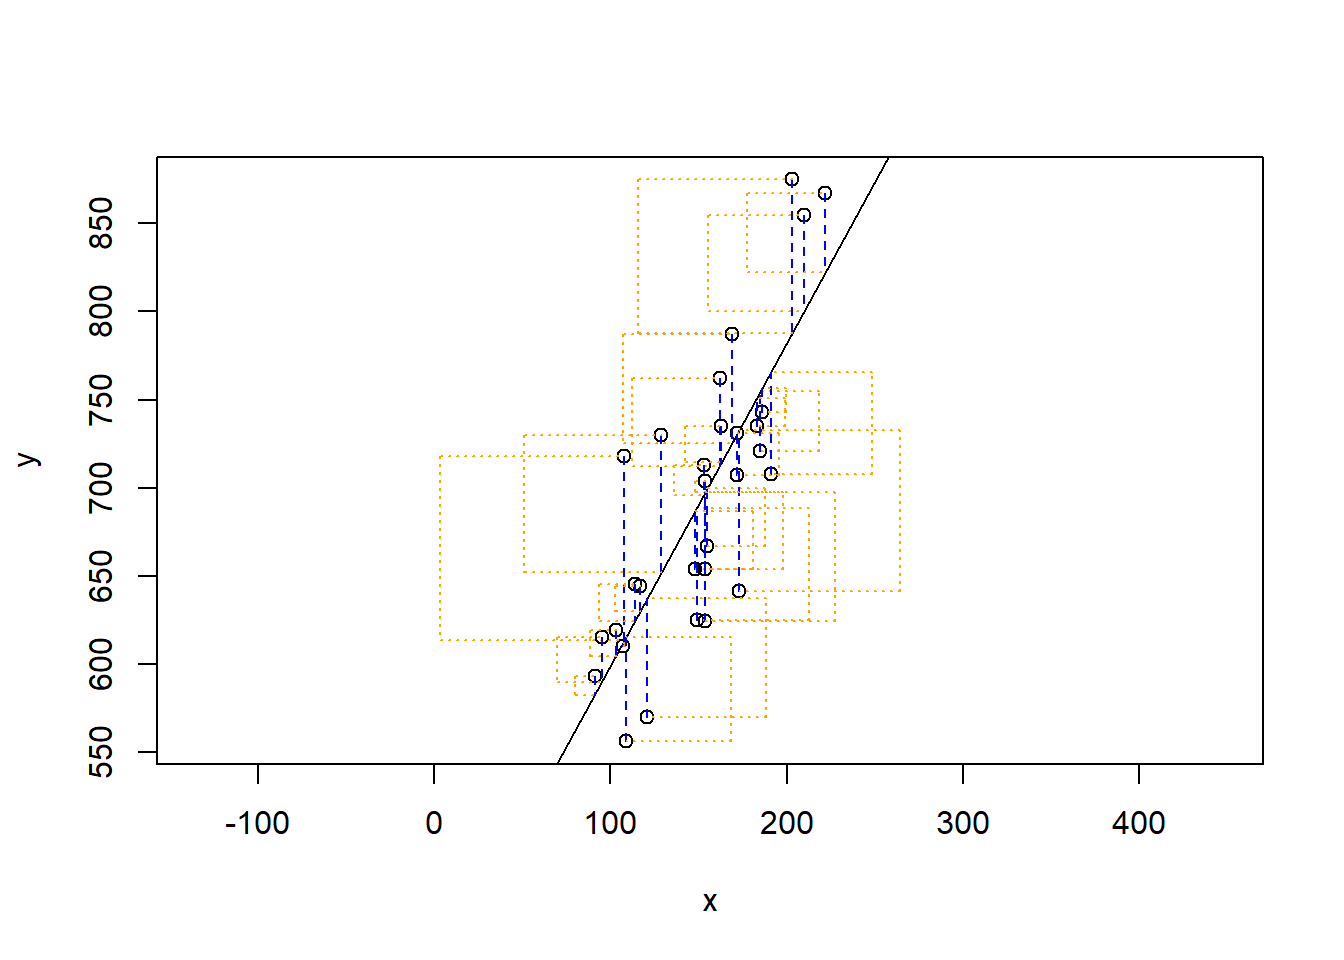
\includegraphics{DATA605_Discussion_13_files/figure-latex/unnamed-chunk-2-1.pdf}

\hypertarget{looking-for-the-value-where-the-point-of-intersection-falls-below-0}{%
\subparagraph{Looking for the value where the point of intersection
falls below
0:}\label{looking-for-the-value-where-the-point-of-intersection-falls-below-0}}

\begin{Shaded}
\begin{Highlighting}[]
\NormalTok{(rootF <-}\StringTok{ }\KeywordTok{uniroot}\NormalTok{(}\ControlFlowTok{function}\NormalTok{(x)  }\KeywordTok{f}\NormalTok{(x) }\OperatorTok{-}\StringTok{ }\KeywordTok{g}\NormalTok{(x)  , }\KeywordTok{c}\NormalTok{(}\OperatorTok{-}\DecValTok{5000}\NormalTok{,}\OperatorTok{-}\FloatTok{0.01}\NormalTok{), }\DataTypeTok{tol=}\FloatTok{1e-8}\NormalTok{)) }
\end{Highlighting}
\end{Shaded}

\begin{verbatim}
## $root
## [1] -2
## 
## $f.root
## [1] 1.776357e-15
## 
## $iter
## [1] 29
## 
## $init.it
## [1] NA
## 
## $estim.prec
## [1] 8.680272e-09
\end{verbatim}

\hypertarget{what-is-the-root-of-the-function}{%
\subparagraph{What is the root of the
function:}\label{what-is-the-root-of-the-function}}

\begin{Shaded}
\begin{Highlighting}[]
\NormalTok{rootF}\OperatorTok{$}\NormalTok{root}
\end{Highlighting}
\end{Shaded}

\begin{verbatim}
## [1] -2
\end{verbatim}

\hypertarget{looking-for-the-value-where-the-point-of-intersection-is-above-0}{%
\subparagraph{Looking for the value where the point of intersection is
above
0:}\label{looking-for-the-value-where-the-point-of-intersection-is-above-0}}

\begin{Shaded}
\begin{Highlighting}[]
\NormalTok{(root0 <-}\StringTok{ }\KeywordTok{uniroot}\NormalTok{(}\ControlFlowTok{function}\NormalTok{(x)  }\KeywordTok{f}\NormalTok{(x) }\OperatorTok{-}\StringTok{ }\KeywordTok{g}\NormalTok{(x)  , }\KeywordTok{c}\NormalTok{(}\FloatTok{0.0001}\NormalTok{, }\DecValTok{5000}\NormalTok{), }\DataTypeTok{tol=}\FloatTok{1e-8}\NormalTok{))}
\end{Highlighting}
\end{Shaded}

\begin{verbatim}
## $root
## [1] 1
## 
## $f.root
## [1] 2.112702e-09
## 
## $iter
## [1] 29
## 
## $init.it
## [1] NA
## 
## $estim.prec
## [1] 5.000001e-09
\end{verbatim}

\hypertarget{what-is-the-root-of-the-function-1}{%
\subparagraph{What is the root of the
function:}\label{what-is-the-root-of-the-function-1}}

\begin{Shaded}
\begin{Highlighting}[]
\NormalTok{root0}\OperatorTok{$}\NormalTok{root}
\end{Highlighting}
\end{Shaded}

\begin{verbatim}
## [1] 1
\end{verbatim}

\hypertarget{therefore-the-area-between-the-curves-will-be-g-minus-f-at-x-2-1}{%
\paragraph{Therefore, the area between the curves will be g minus f at
x(-2,
1)}\label{therefore-the-area-between-the-curves-will-be-g-minus-f-at-x-2-1}}

\hypertarget{integrating-for-g}{%
\subparagraph{integrating for g}\label{integrating-for-g}}

\begin{Shaded}
\begin{Highlighting}[]
\NormalTok{(areaG <-}\StringTok{ }\KeywordTok{integrate}\NormalTok{(g, }\DataTypeTok{lower =} \DecValTok{-2}\NormalTok{, }\DataTypeTok{upper =} \DecValTok{1}\NormalTok{))}
\end{Highlighting}
\end{Shaded}

\begin{verbatim}
## -6 with absolute error < 9.9e-14
\end{verbatim}

\hypertarget{integrating-for-f}{%
\subparagraph{integrating for f}\label{integrating-for-f}}

\begin{Shaded}
\begin{Highlighting}[]
\NormalTok{(areaF <-}\StringTok{ }\KeywordTok{integrate}\NormalTok{(f, }\DataTypeTok{lower =} \DecValTok{-2}\NormalTok{, }\DataTypeTok{upper =} \DecValTok{1}\NormalTok{))}
\end{Highlighting}
\end{Shaded}

\begin{verbatim}
## -10.5 with absolute error < 1.4e-13
\end{verbatim}

\hypertarget{compute-difference-between-g_area-and-f_area}{%
\subparagraph{compute difference between g\_area and
f\_area}\label{compute-difference-between-g_area-and-f_area}}

\begin{Shaded}
\begin{Highlighting}[]
\NormalTok{areaG}\OperatorTok{$}\NormalTok{value }\OperatorTok{-}\StringTok{ }\NormalTok{areaF}\OperatorTok{$}\NormalTok{value}
\end{Highlighting}
\end{Shaded}

\begin{verbatim}
## [1] 4.5
\end{verbatim}


\end{document}
